We developed a new, unified framework for implementing turnover. 
We then simulated a deterministic compartmental model of an illustrative STI,
with turnover as per the framework,
to conduct out experiments.
% SM: consistency & double-checks
%     - avoid using the words 'this', 'these', etc. as much as possible.
%       Used **a lot** throughout methdods section reviewed so far
%     - numbers (3 or three)
%     - (relative) size(s) of risk group(s)
%     - incidence / prevalence among vs in group x
% ==================================================================================================
\subsection{A unified framework for implementing turnover}
\label{ss:framework}
\begin{figure}
  \centering
  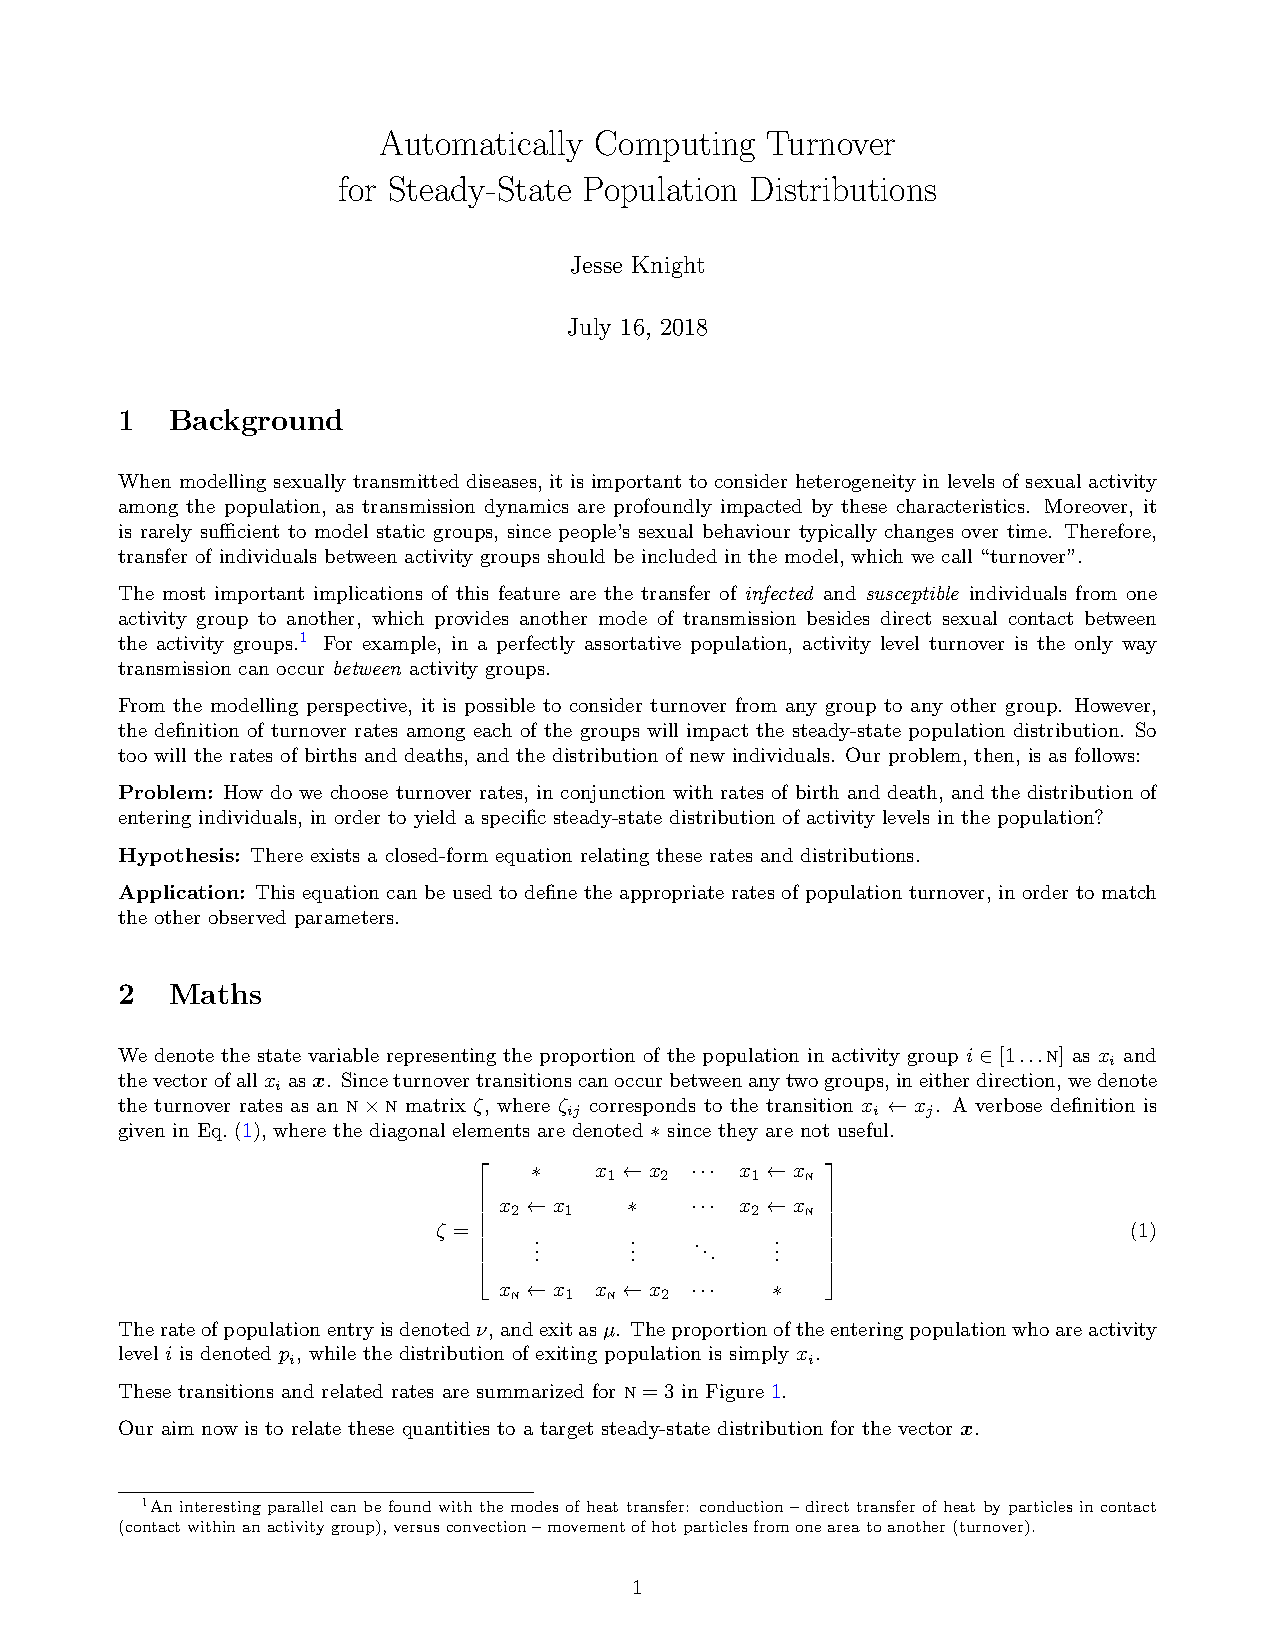
\includegraphics[width=0.5\linewidth]{turnover}
  \caption{System of $G = 3$ risk groups and turnover between them.}
  \footnotesize\raggedright
  $x_i$: number of individuals in risk group~$i$;
  $e_i$: number of individuals available to enter risk group~$i$;
  $\nu$: rate of population entry;
  $\mu$: rate of population exit;
  $\phi_{ij}$: rate of turnover from group~$i$ to group~$j$.
  \label{fig:system}
\end{figure}
We developed a framework for implementing turnover,  
as depicted in Figure~\ref{fig:system}
and detailed in Appendix~\ref{a:framework}. 
In the framework, the simulated population is divided into $G$ risk groups.
The number of individuals in group $i \in [1, \dots, G]$ is denoted $x_i$,
and the relative size of each group is denoted $\hat{x}_i = x_i / N$,
where $N$ is the total population size.
Individuals enter the population at a rate $\nu$ and exit at a rate $\mu$ per year.
The distribution of risk groups at entry into the model
is denoted $\hat{e}_i$, which may be different from $\hat{x}_i$.
The total number of individuals entering group~$i$ per year
is therefore given by $\nu \hat{e}_i N$.
Turnover rates are collected in a $G \times G$ matrix $\phi$,
where $\phi_{ij}$ is the proportion of individuals in group~$i$
who move from group~$i$ into group~$j$ each year.
The framework is independent of the disease model,
and thus transition rates $\phi$ do not depend on health states.
% SM: But health states have not been described yet.
%     Seems funny to write it into the unified system noh?
%     Perhaps should say that the unified system is independent of the disease model,
%     and thus, independent of the health states, or something like that?
% JK: Good point! How is the sentense above?
\par
The framework assumes that:
% SM: Clarify that the 'we assume' part is specific to the research question
%     - i.e. for the set of experiments in the current paper.
%     vs. the unified framework assumes that the relative size of risk groups remain stable, etc.
% JK: Good point. Actually here the assumptions are for the framework overall,
%     then in {sss:turnover-implemented} we add additional assumptions as constraints
%     for the experiments.
1.~the relative sizes of risk groups
$\bm{\hat{x}} = [\hat{x}_1, \dots, \hat{x}_G]$
are known and should remain constant over time; and
2.~the rates of population entry $\nu$ and exit $\mu$
are known, but that they may vary over time.
An approach to estimate $\nu$ and $\mu$ is detailed in Appendix~\ref{aaa:params-nu-mu}.
The framework then provides a method to estimate
the values of the parameters $\bm{\hat{e}}$ and $\phi$,
representing $G$~and~$G(G-1) = G^2$ total unknowns.
In the framework,
$\bm{\hat{e}}$ and $\phi$ are collected in the vector
$\bm{\theta} = \left[\bm{\hat{e}}, \bm{y}\right]$,
where $\bm{y} = \mathrm{vec}_{i \ne j}(\phi)$.
% JK: regarding tense, though we changed this section to past tense recently,
%     I found it confusing to read this section in past tense,
%     since the framework simply exists (in present)
%     and it continutes to "actively" facilitates solving the system.
%     In experiment sections we can describe how we used it (past tense) to do things,
%     but really I think it makes more sense to use present tense for this para.
%     What do you think @SM?
To uniquely determine the elements of $\bm{\theta}$,
a set of linear constraints are constructed.
Each constraint $k$ takes the form
% SM: remove 'this' and 'these' from every sentence in paper,
%     and then put back in with a clear definition of the subject :)
$b_k = A_k \bm{\theta}$,
where $b_k$ is a constant and $A_k$ is a vector with the same length as $\bm{\theta}$.
The values of $\bm{\theta}$ are then obtained by solving:
\begin{equation}\label{eq:system-matrix}
\bm{b} = A \thinspace \bm{\theta}
\end{equation}
using existing algorithms for solving linear systems~\citep{LAPACK}.
\par
The framework defines four types of constraints, which are based on assumptions,
that can used to solve for the values of
$\bm{\hat{e}}$~and~$\phi$ via~$\bm{\theta}$.
The frameworks is flexible with respect to
selecting and combining these constraints,
guided by the availability of data.
However, exactly $G^2$ non-redundant constraints must be specified
to produce a unique solution,
such that exactly one value of $\bm{\theta}$ satisfies all constraints.
Table~\ref{tab:constraints} summarizes
the four types of constraints,
with their underlying assumptions,
and the types of data that can be used in each case.
Additional details, including
constraint equations, examples, and considerations for combining constraints,
are in Appendix~\ref{aaa:params-turnover}.
% SM: hard copy of edits on your desk. the references need some work.
% JK: TODO
\begin{table}
  \centering
  \caption{Summary of constraint types for defining risk group turnover}
  \label{tab:constraints}
  \begin{tabular}{clccl}
	\toprule
	   & Name                       &            Eq.            &        E.g.         & Data requirements                                                         \\
	\midrule
	1. & Constant group size        & (\ref{eq:mass-balance-2}) & (\ref{eq:eg-basis}) & all values of $\hat{x}_i$ and $\nu$                                       \\
	2. & Specified elements         &   (\ref{eq:spec-elem})    & (\ref{eq:eg-spec})  & any value of $\hat{e}_i$ or $\phi_{ij}$                                   \\
	3. & Group duration             & (\ref{eq:duration-group}) &  (\ref{eq:eg-dur})  & any value of $\delta_i$                                                   \\
	4. & Relative rates of turnover &     (\ref{eq:ratio})      & (\ref{eq:eg-ratio}) & any relationship between two turnover rates $\phi_{ij}$ and $\phi_{i'j'}$ \\
	\bottomrule
\end{tabular}\\[1em]
\footnotesize\flushleft
$\nu$:~rate of population entry;
$\phi_{ij}$:~rate of turnover from group $i$ to group $j$;
$\hat{x}_i$:~proportion of individuals in risk group $i$;
$\hat{e}_i$:~proportion of individuals entering into risk group $i$;
$\delta_i$:~average duration spent in risk group $i$.
\end{table}
% ==================================================================================================
\subsection{Transmission model}\label{ss:model-sim}
We developed a deterministic, compartmental model of an illustrative
sexually transmitted infection with 3 risk groups.
We did not simulate a specific pathogen, but rather constructed a biological system
% JK: "selected" sounds like we chose a real one, so "designed/constructed" here?
that included susceptible, infectious, and treated (or recovered/immune) health states.
The transmission model therefore was mechanistically representative of
sexually transmitted infections like
HIV, where effective antiretroviral treatment represents a health state where
individuals are no longer susceptible nor infectious~\citep{Maartens2014}, or
hepatitis B virus, where a large proportion of individuals who clear their acute infection
develop life-long protective immunity~\citep{Ganem2004}.
\par
The model is represented by a set of coupled ordinary differential equations
(Appendix~\ref{aa:eqs-model}) and includes
three health states:
susceptible~$\mathcal{S}$, infectious~$\mathcal{I}$, and treated~$\mathcal{T}$
(Figure~\ref{fig:health-states}),
and $G = 3$ levels of risk:
high~$H$, medium~$M$, and low~$L$.
\begin{figure}
  \centering
  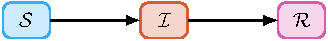
\includegraphics[width=0.4\linewidth]{health-states}
  \caption{Modelled health states:
    $\mathcal{S}$: susceptible;
    $\mathcal{I}$: infected;
    $\mathcal{T}$: treated;
    and transitions:
    $\lambda$: force of infection;
    $\tau$: treatment.}
  \label{fig:health-states}
\end{figure}
Risk strata are defined by different number of partners per year,
so that individuals in risk group~$i$ are assumed to
form partnerships at a rate $C_{i}$ per year.
The probability of partnership formation $\rho_{ik}$ between individuals in group~$i$
and individuals in risk group~$k$ is assumed to be
proportionate to the total number of available partnerships within each group:
\begin{equation}
\rho_{ik} = \frac
{C_k x_k}
{\sum_{\mathrm{k}}C_{\mathrm{k}} x_{\mathrm{k}}}
\label{eq:rho}
\end{equation}
\par
The biological probability of transmission is defined as $\beta$ per partnership.
Individuals transition from the
susceptible $\mathcal{S}$ to infectious $\mathcal{I}$ health state
via a force of infection $\lambda_i$ per year, per susceptible in risk group~$i$:
\begin{equation}
\lambda_{i} =
C_{i} \sum_k \rho_{ik} \thinspace  \beta \thinspace \frac{\mathcal{I}_k}{x_k}
\label{eq:foi}
\end{equation}
Individuals are assumed to transition from the
infectious $\mathcal{I}$ to treated $\mathcal{T}$ health state
at a rate $\tau$ per year, reflecting diagnosis and treatment.
The treatment rate does not vary by risk group.
Individuals in the treated $\mathcal{T}$ health state are neither infectious nor susceptible,
and individuals cannot become re-infected.
% --------------------------------------------------------------------------------------------------
\subsubsection{Implementing turnover within the transmission model}
\label{sss:turnover-implemented}
As described in Section~\ref{ss:framework}, individuals
enter the model at a rate $\nu$,
exit the model at a rate $\mu$,
and transition from risk group~$i$ to group~$j$ at a rate $\phi_{ij}$,
 health state.
The turnover rates $\phi$ and
distribution of individuals entering the model by risk group $\bm{\hat{e}}$
were computed using the methods outlined in
Appendix~\ref{aaa:params-turnover}, based on the following three assumptions.
% SM: assumption, or condition, or constraint? 
% SB: Do we need to explain why we made these assumptions? Or provide refs?
% JK: Since we are constructing a simulated system, I'm not sure what refs might be appropriate,
%     but, you make a great point about justifying.
%     I've added a sentence after all 3 assumptions explaining.
%     I think I was avoiding this because it was hard to explain,
%     but let me know how it reads.
First, we assumed that
the proportion of individuals entering each risk group $\bm{\hat{e}}$
was equal to the proportion of individuals across risk groups in the model $\bm{\hat{x}}$.
% LW: And another strong assumption which was implicit here is that u assume
%     the rate of turn over to be the same irrespective of disease status.
%     And I think it is critical to make it explicit.
%     So S, I, T all have the same turn over rate,
% JK: So, I did now include this in the Turnover System section (last sentence).
%     Do you think it needs to be restated here?
% SM: yes, re-iterate here (before 'first')
% JK: done.
Second, we assumed that
the average duration of time spent in each risk group $\bm{\delta}$ was known.
Third, we assumed that the absolute number of individuals
moving between two risk groups in either direction was balanced,
meaning that if 10 individuals moved from group~$i$ to group~$j$,
then another 10 individuals moved from group~$j$ to group~$i$.
% JK: @SM ^ re. revision above -- this balanced in/out in either direction
%     is not necessary to maintain stable group sizes over time,
%     so I've edited with the example, instead of
%     "such that the proportion of individuals in each risk group remained stable over time".
% SM: yes agree a strong assumption, but one that most models make.
%     So make sure to discuss each of these excellent points by SB and LW and HM in the discussion!
% LW: I would think this is a very strong assumption.
%     It is essentially saying the turn-over system consistently
%     *swap* individuals in two risk groups.
% HM: Not fully understand how does this assumption work?
%     If high risk group has 10 individuals move to medium group,
%     medium group will move 10 individuals to high risk? This is independent from population entry?
% JK: @HM: yes, this is what this assumption means. I've edited hopefully to be more clear.
% SM: could be more clear. suggest giving an example  as HM did in her comments.
%     @LW: see new sentence below. We have to make at least one more assumption,
%     else the system will not have a unique solution,
%     and by "balancing" the turnover rates, it is a way of avoiding "bias":
% JK: done -- thanks team for the strong detail!
These three assumptions were selected
because they reflect the common assumptions underlying turnover in prior models
\citep{Zhang2012,Henry2015}
and also to avoid any dominant direction of turnover.
That is, we wanted to study
the influence of movement between risk groups in general,
as compared to no movement, and at various rates of movement,
rather than movement predominantly from some groups to some other groups.
The system of equations formulated from the above assumptions and constraints
is given in Appendix~\ref{aa:eqs-turnover}.
To satisfy all three assumptions, there was only one possible value
for each element in $\phi$~and~$\bm{\hat{e}}$.
That is, by specifying these three assumptions,
we generated a unique set of $\phi$~and~$\bm{\hat{e}}$.
\par
% SM: I did not understand the paragraph below.
Under the above three assumptions,
we still needed to specify the particular values of the parameters
$\bm{\hat{x}}$,~$\bm{\delta}$,~$\nu$,~and~$\mu$.
Such parameter values could be derived from data as described in Appendix~\ref{aaa:params-turnover}.
However, in all our experiments, we used the illustrative values summarized in
Table~\ref{tab:params}.
% LW: After read the whole results section,
%     I think experiment 2 and 3.2 followed values specified in Table 3.
%     But experiment 1 and 3.1 explored a wide range of
%     turn-over and treatment rates.
%     it is unclear what do u refer to when u said “this experiment”.
%     Given the organization and length – by the time I reached results of Experiemnt 2,
%     I almost forgot under which values they were done – as the section preceed it
%     explored a range of values of turn-over rate and treatment rate.
% JK: Hopefully now with the paper much much shorter, this is resolved?
After resolving the system of equations Eq.~(\ref{eq:system-matrix}) using these values,
$\bm{\hat{e}}$ was equal to $\bm{\hat{x}}$ (assumed), and $\phi$ was:
\begin{equation}
\label{eq:phi-values}
\phi = \left[\begin{array}{ccc}
* & 0.0833 & 0.0867\\
0.0208 & * & 0.0158\\
0.0058 & 0.0042 & *
\end{array}\right]

\end{equation}
\begin{table}
  \centering
  \caption{Default model parameters for experiments}
  \label{tab:params}
  \begin{tabular}{clc}
	\toprule
	    Symbol     & Description                                                     &            Value             \\
	\midrule
	 $\bm{\beta}$  & transmission probability per contact                            &            $0.03$            \\
	    $\tau$     & rate of treatment initiation among infected                     &            $0.1$             \\
	    $N_0$      & initial population size                                         &            $1000$            \\
	\midrule
	$\bm{\hat{x}}$ & proportion of system individuals by risk group                  & $[ 0.05 \es 0.20 \es 0.75 ]$ \\
	$\bm{\hat{e}}$ & proportion of entering individuals risk by risk group           & $[ 0.05 \es 0.20 \es 0.75 ]$ \\
	$\bm{\delta}$  & average duration spent in each risk group                       &    $[ 5 \es 15 \es 25 ]$     \\
	     $C$       & rate of contact formation among individuals in each risk group  &     $[ 25 \es 5 \es 1 ]$     \\
	    $\nu$      & rate of population entry                                        &            $0.05$            \\
	    $\mu$      & rate of population exit                                         &            $0.03$            \\
	\bottomrule
\end{tabular}
  % SS: All of this seems a little hard to follow in terms of the infection,
  %     b/c it seems to indicate that there is an underlying infection of interest,
  %     but it is not being stated.
  % JK: Same as above, not sure what to say here...
  %     We did start out with HIV, but since we're not considering STI-mortality,
  %     we really cannoy call it HIV.
\end{table}
We then simulated epidemics using $\phi$ above
and the parameters shown in Table~\ref{tab:params}.
The transmission model was initialized with $N_0 = 1000$ individuals
who were distributed across risk groups according to $\bm{\hat{x}}$.
We seeded the epidemic with
one infectious individual in each risk group at $t = 0$ in an otherwise 
fully susceptible populatuon.
We numerically solved the system of ordinary differential equations
(Appendix~\ref{aa:eqs-model}) in Python
using Euler's method with a time step of $dt = 0.1$ years.
Code for all aspects of the project is available at:
\href{https://github.com/c-uhs/turnover}{\small\texttt{https://github.com/c-uhs/turnover}}.
% ==================================================================================================
\subsection{Experiments}
\label{ss:exp}
We designed three experiments to examine the influence of turnover on simulated epidemics.
We analyzed all outcomes at equilibrium,
defined as steady state at $t = 500$ years
with $<1\%$ change in incidence per year.
% --------------------------------------------------------------------------------------------------
\subsubsection{Experiment~1: Mechanisms by which turnover influences equilibrium prevalence}
\label{sss:exp-prevalence}
We designed Experiment~1 to explore the mechanisms by which turnover influences
the equilibrium STI prevalence of infection, and
the ratio of prevalence between risk groups (prevalence ratios).
We defined prevalence as $\hat{\mathcal{I}}_i = \dfrac{\mathcal{I}_i}{x_i}$.
%and incidence as $\lambda_i$ from Eq.~(\ref{eq:foi}).
Similar to previous studies \citep{Zhang2012,Henry2015},
we varied the rates of turnover using a single parameter.
However, because our model had $G = 3$ risk groups,
multiplying a set of base rates $\phi$ by a scalar factor
would change the relative population sizes of risk groups~$\bm{\hat{x}}$.
Instead of a scalar factor, we controlled the rates of turnover using
the duration of time spent in the high risk group~$\delta_H$,
because of the practical interpretation of $\delta_H$
in the context of STI transmission,
such as the duration in formal sex work \citep{Watts2010}.
A shorter $\delta_H$ yielded faster rates of turnover among all groups.
% SM: implied or means or is equivalent to? 'implied' seems vague?
% JK: changed to 'yielded' - @SM is that better?
The duration of time spent in the medium risk group $\delta_M$
was then defined as a value between $\delta_H$ and the maximum duration $\mu^{-1}$
which scaled with $\delta_H$ following:
$\delta_M = \delta_H + \kappa \left(\mu^{-1} - \delta_H\right)$, with $\kappa = 0.3$.
The duration of time in the low risk group $\delta_L$
similarly scaled with $\delta_H$,
but due to existing constraints,
specification of $\delta_H$ and $\delta_M$
ensured only one possible value of $\delta_L$.
Thus, each value of $\delta_H$ yielded a unique set of turnover rates~$\phi$
whose elements all scaled inversely with
the duration in the high risk group~$\delta_H$.
\par
We varied $\delta_H$ across a range of 33~to~3 years,
reflecting a range from
the full duration of simulated sexual activity $\mu^{-1} \approx 33$ years,
through an average reported duration in sex work as low as 3 years
\citep{Watts2010}.
The resulting duration of time spent in each group
versus turnover in the high risk group $\delta_H^{-1}$
is shown in Figure~\ref{fig:dur-group}.
\begin{figure}
  \centering\includegraphics[width=0.45\linewidth]{{1d-dur-all-tau=0.1}.pdf}
  \caption{Average duration of time spent in each risk group versus turnover.
    Turnover rate (log scale) is a function of
    the duration of time spent in the high risk group $\delta_H$,
    where shorter time spent in the high risk group yields faster turnover.}
  \label{fig:dur-group}
\end{figure}
For each set of turnover rates,
we plotted the equilibrium prevalence in each risk group,
and the prevalence ratios between high/low, high/medium, and medium/low risk groups.
In order to understand the mechanisms by which
turnover influenced prevalence and prevalence ratios (Objective~1),
we additionally plotted the four components which contributed to
gain/loss of infectious individuals in each risk group,
based on Eq.~(\ref{eq:model-I}):
1)~net gain/loss via turnover of infectious individuals,
2)~gain via incident infections,
3)~loss via treatment, and
4)~loss via death.
The influence of turnover on prevalence
was only mediated by components 1~and~2,
since components 3~and~4 were defined as
constant rates which did not change with turnover;
as such, our analysis focused on components 1~and~2.
Finally, to further understand trends in incident infections versus turnover (component~1),
we factored equation Eq.~(\ref{eq:foi}) for incidence $\lambda_i$
into constant and non-constant factors,
and plotted the non-constant factors versus turnover.
% --------------------------------------------------------------------------------------------------
\subsubsection{Experiment~2: Inferred risk heterogeneity with vs without turnover}
\label{sss:exp-infer}
We designed Experiment~2 to examine how
the inclusion versus exclusion of turnover influences
the inference of transmission model parameters related to risk heterogeneity,
specifically the numbers of partners per year $C_i$ across risk groups.
The ratio of partner numbers $C_H~/~C_L$
is one way to measure of how different the two risk groups are
with respect to acquisition and transmission risks.
Indeed, ratios of partner numbers are often used when parameterizing 
risk heterogeneity in STI transmission models \citep{Mishra2012}.
\par
First, we fit the transmission model with turnover and without turnover,
to equilibrium infection prevalence across risk groups.
Specifically, we held all other parameters at their default values and
fit the numbers of partners per year in each risk group $C_i$
to reproduce the following:
20\% infection prevalence among the high risk group,
8.75\% among the medium risk group,
3\% among the low risk group,
and 5\% overall.
To identify the set of parameters (i.e.\ partner numbers $C$ in each risk group)
that best reproduced the fitting targets, we minimized
the negative log-likelihood of group-specific and overall prevalence.
Sample sizes of 500, 2000, 7500, and 10,000 were assumed to generate binomial distributions
for the high, medium, low, and overall prevalence targets respectively,
reflecting typical sample sizes in
nationally representative demographic and health surveys \citep{DHS},
multiplied by the relative sizes of risk groups in the model~$\bm{\hat{x}}$.
The minimization was performed using
the SLSQP method~\citep{Kraft1988} from the SciPy Python
\href{https://docs.scipy.org/doc/scipy/reference/generated/scipy.optimize.minimize.html}
{\texttt{minimize}} package.
To address Objective~2, we compared
the fitted (posterior) ratio of partners per year $C_H~/~C_L$
% SM: in introduction, helpful if objectives listed.
% JK: done.
in the model with turnover versus the model without turnover.
% --------------------------------------------------------------------------------------------------
\subsubsection{Experiment~3: Influence of turnover on the tPAF of the high risk group}
\label{sss:exp-tpaf}
We designed Experiment~3 to examine how the tPAF of the
high risk group varies when estimated
by a model with versus without turnover (Objective~3).
We calculated the tPAF of risk group~$i$ by comparing
the relative difference in cumulative incidence between
a base scenario, and a counterfactual where transmission from group~$i$ is turned off,
starting at the fitted equilibrium.
That is, in the counterfactual scenario,
infected individuals in the high risk group could not transmit the infection.
The tPAF was calculated over different time-horizons (1~to~50 years) as
\citep{Mishra2014}:
\begin{equation}
\textrm{tPAF}_i(t) =
  \frac{\displaystyle\int_{t_{eq}}^{t} I_b(\tau) \, d\tau -
        \displaystyle\int_{t_{eq}}^{t} I_c(\tau) \, d\tau}
       {\displaystyle\int_{t_{eq}}^{t} I_b(\tau) \, d\tau}
\end{equation}
where $t_{eq}$ is the time corresponding to equilibrium,
$I_b(t)$ is the rate of new infections at time $t$ in the base scenario,
and $I_c(t)$ is the rate of new infections at time $t$ in the counterfactual scenario.
We then compared the tPAF generated from the fitted model with turnover
to the tPAF generated from the fitted model without turnover.
